\documentclass{article}

% if you need to pass options to natbib, use, e.g.:
% \PassOptionsToPackage{numbers, compress}{natbib}
% before loading nips_2017
%
% to avoid loading the natbib package, add option nonatbib:
% \usepackage[nonatbib]{nips_2017}

\usepackage[final]{nips_2017}


\usepackage[utf8]{inputenc} % allow utf-8 input
\usepackage[T1]{fontenc}    % use 8-bit T1 fonts
\usepackage{hyperref}       % hyperlinks
\usepackage{url}            % simple URL typesetting
\usepackage{booktabs}       % professional-quality tables
\usepackage{amsfonts}       % blackboard math symbols
\usepackage{nicefrac}       % compact symbols for 1/2, etc.
\usepackage{microtype}      % microtypography

\usepackage{array,booktabs,tabularx}
\usepackage{amsmath}        % text in math mode
\usepackage[colorinlistoftodos,prependcaption,textsize=tiny]{todonotes}
\renewcommand{\arraystretch}{1.2}

% Choose a title for your submission
\title{Story Cloze Test Project Report}

\author{
  Thomas Diggelmann\\
  ETH Zurich\\
  \texttt{thomasdi@student.ethz.ch}\\
  \And
  Doruk Cetin\\
  ETH Zurich\\
  \texttt{dcetin@student.ethz.ch}\\
  \And
  George Mtui\\
  ETH Zurich\\
  \texttt{gmtui@student.ethz.ch}\\
}

\begin{document}
% \nipsfinalcopy is no longer used

\maketitle

% We do not requrire you to write an abstract. Still, if you feel like it, please do so.
%\begin{abstract}
%\end{abstract}

\section{Introduction}
One end goal of Natural Language Understanding (NLU) as a branch is to develop systems that can understand structure and meaning of the human languages. The NLU community has achieved milestones in many application areas such as sentiment analysis, machine translation and question answering. As the evaluation of NLU systems are hard, researches have been designing proxy tasks for many subfields to train and evaluate such systems.

\par We tackle one such task, named Story Cloze Test (SCT) \citep{mostafazadeh2016corpus}, which considers story understanding to assess systems' capabilities of reading comprehension. The authors introduce the ROCStories corpus, where each entry is a five-sentence commonsense story. The SCT framework is defined on this corpus, where they randomly sampled a subset of the stories and created couples of \textit{right} and \textit{wrong} endings (with respect to their plausibility, entailment and relevance) on top of their four-sentence contexts. Here, a system is expected to choose between a right and a wrong ending, given four preceding sentences as the context.

\par Authors \citep{mostafazadeh2017lsdsem} report results from eight systems on SCT and discuss the interesting outcomes of different approaches. Previous baseline on the task was improved from $58.5\%$ to $75.2\%$. One major complication of the SCT is the lack of negative examples in the training data, as the corpus only contains stories with correct endings. \citet{roemmele2017rnn} and \citet{bugert2017lsdsem} choose to generate fake incorrect examples by sampling through endings from the training corpus itself and \citet{wang2017conditional} use a GAN to generate fake endings. However, models that are trained only using the training dataset achieved significantly less accuracies than the ones that utilized validation data (which has both positive and negative examples) in training. One such extreme case is explored in \citet{schwartz2017effect}, where they completely ignore the context sentences and train a model on the features extracted only from the validation dataset, which achieved a surprising accuracy score of $72.4\%$. Similarly, \citet{mostafazadeh2017lsdsem} claim sentiment is one factor in correct detection along with the stylistic features isolated in ending sentences. Since the task was not conducted as a blind challenge, it is not clear if the aforementioned methods capture artifacts of the test set and whether they can generalize well to unseen data.

\section{Methodology \& Model}
We wanted to implement a model where we do not leverage the implicit biases (c.f. effects of directly using sentiment and stylistic features) but keep as close as possible to the original intent of the SCT. Our approach is to train a robust language model (LM) on the training dataset, with the help of multi-task learning, to indirectly integrate knowledge about sentiment. Our aim is to obtain a model that ``understands” the text rather than relying on the stylistic differences in the validation corpus.

\begin{figure}[htbp]
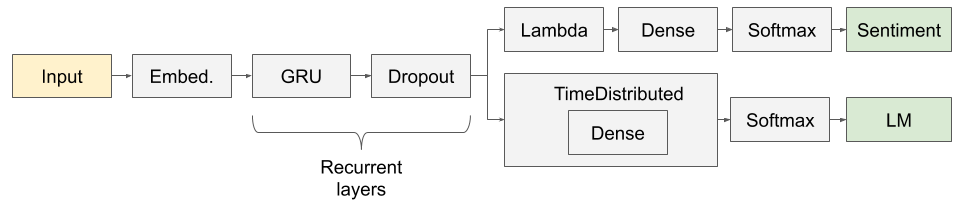
\includegraphics[width=\textwidth]{nlu_model.png}
\centering
\caption{Architecture of the multi-task learning model, which additionally uses sentiment prediction as a second task besides the classic RNN-predict-next-word language model task.}
\label{fig:model}
\end{figure}

\par Our system is generative in nature: we train a language model on the training dataset and do predictions on the probabilities generated by the LM. Figure \ref{fig:model} illustrates the architecture of our model. The LM is modeled by a recurrent neural network (RNN) that utilizes word embeddings. Sentiment information is only used in the multi-task training of the language model. Lambda layer is used to retrieve the final output of the RNN to base the sentiment prediction.

\par There have previously been a few approaches to incorporate language models to SCT. \citet{roemmele2017rnn} used language models to generate fake endings on the training dataset. \citet{chaturvedi2017story} and \citet{peng2017joint} trained semantic language models to generate conditional probabilities of the sentence sequences, which are incorporated into the final predictor as features. Lastly, \citet{schwartz2017effect} trained a recurrent neural network language model, which they combine with the extracted stylistic features to reach the state of the art in \citet{mostafazadeh2017lsdsem}. Our work follows most closely the work done on language models by \citet{schwartz2017effect}.

\par We test with three different ways to predict the right endings using the outputs of our model. First method is quite straightforward: we compare the output perplexities and classify the ending that generates smaller perplexity as the right one. Second method uses the comparison of the probability ratios, as it is motivated by \citet{schwartz2017effect}. Probabilities are calculated as in the Equation \ref{eqn:proba-ratio}, where we classify ending with high probability as the right ending. The intuition is again the right ending should be less surprising than the wrong one: numerator denotes how unsurprising is the ending given the first four sentences, whereas the denominator accounts for the rare endings sentences that are inherently surprising. Lastly, we train classifiers on the validation dataset, using the features extracted by our trained language models. In other words, we evaluate our model on the validation dataset \textemdash producing sentiment predictions, probabilities and hidden states \textemdash and use the resulting ``features" as input to a classifier to be trained on the validation dataset.
\begin{equation} \label{eqn:proba-ratio}
    \frac{ p_{\theta} (\text{ending} \mid \text{story}) }
    {p_{\theta} (\text{ending}) }
\end{equation}

\section{Training}
In the preprocessing step we convert all the words into lowercase and tokenize them using nltk package. During tokenization, we use a maximum sequence length of 90 words and (pre-)pad all shorter sequences using a prespecified <pad> token. Similarly to \citet{schwartz2017effect}, we use a maximum vocabulary size of 20000. Both of these preprocessing steps are done due to computational reasons. Our models utilize the GloVe embeddings \citep{pennington2014glove} as the embedding layer of the network. Specifically, our experiments use 100 dimensional ``glove.6B" embeddings.

\par We use the VADER \citep{hutto2014vader} sentiment analysis tool to obtain polarity scores for the sentences. We discretize the polarity scores by the typical thresholds suggested by the authors: we classify it as neutral statement if the compound score is in between $(-0.05, 0.05)$, if it is either above or below that interval we classify it as positive or negative sentiment, respectively.

\par We use a compound loss as our objective function as mentioned above. It is simply the weighted average of the two multi-task losses: the language model loss and the sentiment classification loss. Adam optimizer is used to optimize the parameters of our network.

\section{Experiments}
We ran all models for 5 epochs and created model checkpoints after each epoch. We then evaluate the performances of the models on the test set by using their respective best checkpoint on the validation dataset. We use a learning rate of $0.001$ over mini-batches of size $50$ and the dropout rate is consistently $0.5$ for all the models. All experiments are ran on GeForce GTX 1080 Ti on ETH Leonhard cluster. Table \ref{tab:results} summarizes the results of different models on validation and test datasets using different evaluation strategies explained in the previous section. Names denote the number of GRU layers and their respective number of units, e.g. $3x512$ stands for three layers of GRUs with 512 units each.

\begin{table}[htbp]
\centering
\begin{tabularx}{\textwidth}{X|cc|ccc}
\toprule
                        & \multicolumn{2}{c|}{Validation Accuracy}  & \multicolumn{3}{c}{Test Accuracy}                           \\
Model                   & Perplexity          & Prob. Ratio         & Perplexity         & Prob. Ratio        & Features          \\ \hline
1x512                   & 0.548370            & 0.648316            & 0.547301           & 0.639230           & 0.672367          \\
1x512 (w/o sentiment)   & 0.539284            & 0.631213            & 0.538215           & 0.629075           & 0.681988          \\
1x512 (7/3)             & 0.541422            & \textbf{0.649920}   & 0.548370           & \textbf{0.645644}  & \textbf{0.691608} \\
1x512 (attention)       & 0.538215            & 0.637092            & \textbf{0.548904}  & 0.625869           & 0.669695          \\
1x512 (7/3, attention)  & \textbf{0.548904}   & 0.627472            & 0.546232           & 0.632817           & 0.687332          \\
2x1000                  & 0.535008            & 0.637627            & 0.548370           & 0.626937           & 0.687332          \\
3x512                   & 0.540887            & 0.636024            & 0.543025           & 0.630144           & 0.669695          \\
\bottomrule
\end{tabularx}
\label{tab:results}
\caption{Validation and test accuracy scores of different configurations of our architecture}
\end{table}

\par We keep the general architecture introduced in Figure \ref{fig:model} intact and make small modifications. Unless specified, the models use an equal weighting of the loss functions while training. Ratios in parentheses denote the weight factors of language model and sentiment losses, respectively. For some models we replace the lambda layer with a weighted attention layer (\href{https://pypi.org/project/keras-self-attention/}{source}) over the word sequences. We also experiment with deepening the network by replicating the RNN-Dropout layers. We always use GRU as the recurrent cell implementation as our experiments with LSTM (not shown here) did not bring any improvement.

\par Multiple RNN layers slightly under-performed the one layer models, so we choose to stick to a single layer of recurrent units. We have observed that weighting the language model loss more than the sentiment loss helped the model to learn more useful representations of the data. This is in line with our expectations as the LM loss represents our main objective and the sentiment prediction proved to be comparably an easier of a task; all models achieved over $0.98$ accuracy when predicting sentiments over the validation dataset. Still, we can confirm the addition of the sentiment is beneficial and the improvement due to it cannot be ignored. Attention could not improve upon the results of the rather simplistic Lambda layers. We believe this trend \textemdash together with the fact that most of the changes only result in marginal differences \textemdash shows that we already utilize what we can mostly infer from our training setup (i.e. training data, embeddings and sentiment classes).

\begin{figure}[htbp]
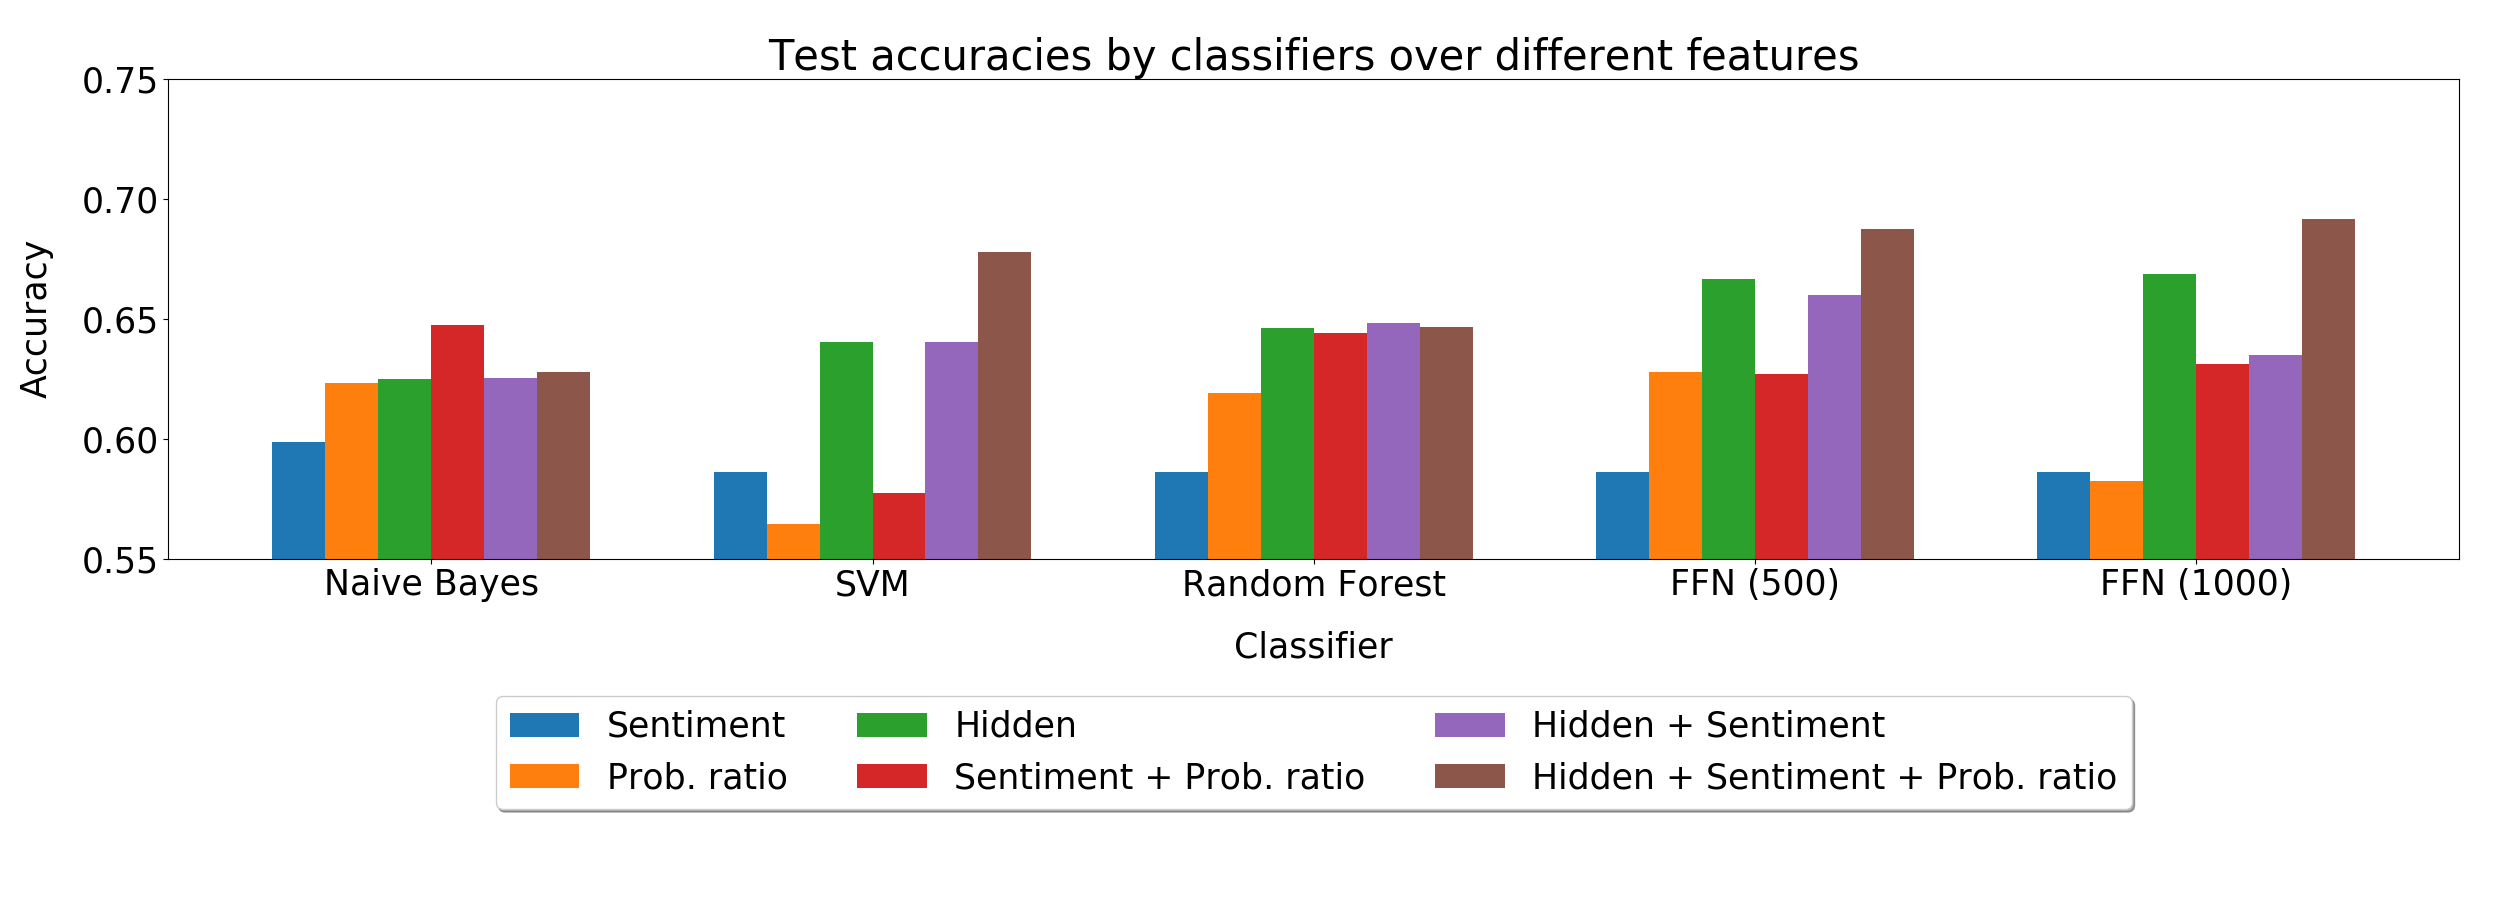
\includegraphics[width=\textwidth]{plot_wide.png}
\centering
\caption{Comparison of the different classifiers trained on different subsets of features. FFN stands for ``feedforward network" and the number inside the parentheses denote the width of their only hidden layer. Results are from the $7/3$ weighted run without attention, arguably our best model.}
\label{fig:classifier-res}
\end{figure}

\par Lastly, Figure \ref{fig:classifier-res} illustrates the third evaluation method. While interestingly probability based classifiers cannot utilize the given features well, SVMs and neural networks can obtain competitive scores on the test set. We can also observe the hidden representations being the most informative set of features, proving it to be very useful for even relatively simple classifiers.

\section{Future Work}
As an extension of the current model, one could also think of integrating further tasks to the multi-tasking approach, such as named entity recognition (NER) or part-of-speech (PoS) tagging. We also believe replacing our ``vanilla LM" with a semantic one that encodes more prior knowledge (e.g. through frame semantics, hierarchical relationships) can lead to models that are more capable at reading comprehension. Similarly, replacing the embedding layer with more powerful word embeddings that are trained on larger corpora could be beneficial to the model.

\section{Conclusion}
We have trained a language model for the Story Cloze Task through multi-task learning, using sentiment polarity scores. Together with the previous studies on the task we have shown that incorporating semantic elements helps the model in reading comprehension, while staying true to the spirit of the task. Although we have trained a generative model to solve this task by proxy, we also confirm that the learned hidden representations can be further exploited by discriminative models.
\par We are providing the predictions on the LM output using probability ratio evaluation method, rather than using the classifier output on extracted features which achieves higher accuracy on test data. We are not after a SOTA result in terms of accuracy but rather wanted to see if we could use an agnostic model that learns from the data and background knowledge.

\bibliographystyle{plainnat}
\bibliography{refs}

\end{document}
